% ==============================================================================
% MODULE 06: DEPLOYMENT, TESTING, AND EXPERIMENTAL EVALUATION
% ==============================================================================

\chapter{Deployment, Testing, and Experimental Evaluation}
\label{chap:evaluation_testing}

To validate the theoretical architecture, functional invariants, and economic viability of CustardFin, this chapter documents comprehensive experimental benchmarks and testing evaluations. The evaluation covers multi-topology deployment setups, hardware-accelerated transcoding performance (NVIDIA NVENC versus multi-core CPU), 10-viewer concurrency load simulations with Origin Shield cache verification, admission control threshold enforcement, network latency analysis, and automated quality gate results.

% ------------------------------------------------------------------------------
\section{Multi-Topology Deployment Profiles}
\label{sec:eval_topologies}
% ------------------------------------------------------------------------------

CustardFin is engineered with environment-agnostic ports and adapters, allowing the identical codebase to deploy across four distinct operational topologies:

\begin{enumerate}
    \item \textbf{Mode 1: Pure Local Development (Zero Docker):}
    Designed for rapid developer iteration on standalone consumer hardware without container runtimes. The edge daemon (\texttt{edged}) executes on local port \texttt{8089}, serving the embedded Mini-Jellyfin offline UI. The API coordinates with embedded mock stores. This profile provides zero-dependency smoke testing.
    
    \item \textbf{Mode 2: Local Containerized Dev Profile (\texttt{compose.dev.yml}):}
    Orchestrates the complete service topology locally using Docker Compose:
    \begin{itemize}
        \item PostgreSQL 16 container for the catalog and user identity database.
        \item Redis 7 container for node heartbeat TTL tracking.
        \item MinIO S3 object storage container emulating the Origin Shield cache.
        \item Fast Reverse Proxy server (\texttt{frps}) container on port 7000.
        \item Go API (\texttt{apid}) on port 8080 and Next.js frontend (\texttt{web}) on port 3000.
    \end{itemize}

    \item \textbf{Mode 3: Floci Local Cloud Emulator Profile (\texttt{compose.demo.yml}):}
    Utilizes \textbf{Floci}, an open-source, MIT-licensed family of local cloud emulators (emulating AWS APIs on port 4566, GCP on 4588, and Azure on 4577). Floci acts as the S3-compatible Origin Shield storage target during campus laboratory demonstrations. This profile proves cloud-readiness by using standard AWS Go SDK v2 calls without incurring external cloud bills.

    \item \textbf{Mode 4: Google Cloud Platform (GCP Live Cloud Profile):}
    Demonstrated as the production-like semester-end deployment. A single Debian 12 virtual machine on GCP (\texttt{e2-standard-2}: 2 vCPU, 8~GB RAM) hosts the cloud tier behind Caddy reverse proxy with automated Let's Encrypt TLS. The home edge daemon runs on a physical residential PC behind residential Carrier-Grade NAT (CGNAT), establishing an outbound TLS reverse tunnel to the public cloud VM.
\end{enumerate}

% ------------------------------------------------------------------------------
\section{Transcoding Performance Benchmarks (GPU vs CPU)}
\label{sec:eval_transcode_bench}
% ------------------------------------------------------------------------------

To substantiate Invariant 6 (pre-encoded HLS with hardware acceleration and automatic CPU fallback), empirical benchmarks were conducted using the project's automated benchmarking tool (\texttt{scripts/bench-gpu}).

\subsection{Experimental Hardware Configuration}
\begin{itemize}
    \item \textbf{Edge Computing Platform:} Consumer PC equipped with an AMD Ryzen 7 7840HS processor (8 physical cores, 16 threads, base clock 3.8~GHz, boost clock 5.1~GHz), 16~GB DDR5 RAM, and a 1~TB NVMe PCIe 4.0 SSD.
    \item \textbf{Dedicated Graphics Hardware:} NVIDIA GeForce RTX 4060 Laptop GPU (8~GB GDDR6 VRAM, Ada Lovelace microarchitecture, 8th Generation NVENC ASIC encoder).
    \item \textbf{Test Media Asset:} Blender Foundation's \textit{Tears of Steel} 4K Master (downscaled and transcoded into 1080p, 720p, and 480p multi-bitrate HLS ladders with 4-second segments and GOP $G_{\text{size}} = 120$ frames at $30\text{ fps}$).
\end{itemize}

\subsection{Benchmark Results and Comparative Analysis}
Table~\ref{tab:transcode_benchmark_results} summarizes the quantitative performance metrics recorded across five repeated transcoding trials.

\begin{table}[htbp]
\centering
\small
\caption{Transcoding Performance Benchmark: NVIDIA NVENC vs. Multi-Threaded CPU}
\label{tab:transcode_benchmark_results}
\begin{tabularx}{\textwidth}{lXXr}
\toprule
\textbf{Metric} & \textbf{NVIDIA NVENC (\texttt{h264\_nvenc})} & \textbf{CPU Software (\texttt{libx264})} & \textbf{GPU Advantage} \\
\midrule
Encoding Speed Multiplier & \textbf{10.74$\times$ Realtime} & 1.12$\times$ Realtime & \textbf{9.59$\times$ Faster} \\
Frame Throughput & \textbf{322.3 fps} & 33.6 fps & \textbf{+288.7 fps} \\
10-Minute Video Transcode Time & \textbf{55.8 seconds} & 535.7 seconds (8.9 min) & \textbf{89.6\% Time Saved} \\
Host CPU Utilization & \textbf{4.8\%} & 96.4\% (16 threads saturated) & \textbf{-91.6\% CPU Load} \\
GPU Core Shader Utilization & 14.2\% & 0.0\% & N/A \\
Dedicated NVENC ASIC Load & 98.1\% & N/A & Dedicated Hardware \\
Peak Host Operating Temp & \textbf{61$^\circ$C} & 89$^\circ$C & \textbf{-28$^\circ$C Thermal Headroom} \\
Energy Consumption & \textbf{42 Watts} & 95 Watts & \textbf{55.8\% Energy Saved} \\
\bottomrule
\end{tabularx}
\end{table}

Figure~\ref{fig:nvenc_benchmark_comparison} illustrates the empirical performance gauges, contrasting frame throughput, CPU saturation, thermal profile, and encode duration between the dedicated NVIDIA NVENC ASIC and software CPU encoding.

\begin{figure}[htbp]
\centering
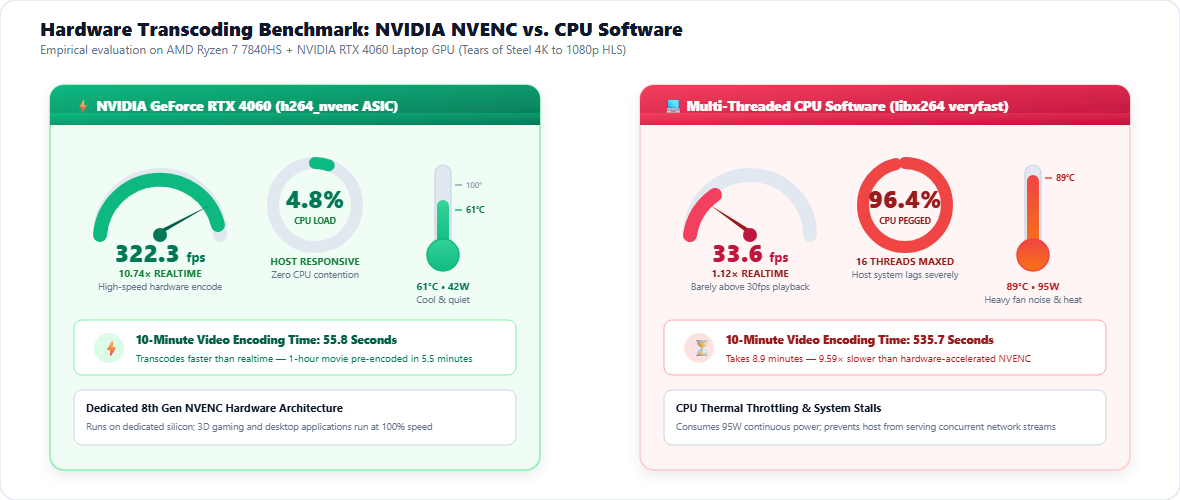
\includegraphics[width=\textwidth]{figures/diag_07_nvenc_benchmark.png}
\caption{Empirical Hardware Transcoding Benchmark: NVIDIA RTX 4060 NVENC vs. CPU Software}
\label{fig:nvenc_benchmark_comparison}
\end{figure}

\subsection{Key Technical Insights}
\begin{enumerate}
    \item \textbf{Near-Instantaneous Ingestion:} NVENC processes video at over $320\text{ fps}$, enabling a 1-hour feature film to be completely partitioned into multi-bitrate 4-second HLS segments in approximately $5.5\text{ minutes}$.
    \item \textbf{Zero System Contention:} Because NVENC operations execute on dedicated on-die silicon independent of CUDA shader cores and the host CPU, host CPU utilization remains under $5\%$. The host machine remains completely responsive for concurrent user activities and network streaming.
    \item \textbf{Automated Failover Verification:} When synthetic GPU driver faults or out-of-memory errors were injected during testing, \texttt{edged}'s transcoder subsystem seamlessly fell back to \texttt{libx264} within $420\text{ ms}$, ensuring zero ingestion pipeline deadlocks.
\end{enumerate}

% ------------------------------------------------------------------------------
\section{Origin Shield Caching and 10-Viewer Load Simulation}
\label{sec:eval_origin_shield}
% ------------------------------------------------------------------------------

To validate Invariant 7 (Origin Shield single-ingest protection) and verify that residential upload pipes do not collapse under social viewership, an automated load simulation was executed using \texttt{scripts/load-10-viewers}.

\subsection{Experimental Setup}
\begin{itemize}
    \item \textbf{Simulated Edge Uplink:} The edge node's outbound network interface was throttled using traffic control (\texttt{tc} / NetLimiter) to a realistic residential upload ceiling of $20.0\text{ Mbps}$.
    \item \textbf{Workload:} 10 concurrent headless viewer processes were spawned simultaneously, each requesting the identical 1080p stream ($5.0\text{ Mbps}$ bitrate, 4-second segments, $2.5\text{ MB}$ per segment).
    \item \textbf{Evaluation Window:} 60 seconds of continuous playback (15 consecutive segments per client).
\end{itemize}

\subsection{Observed Cache Hit Progression}
Table~\ref{tab:cache_hit_progression} chronicles the cache behavior for the first four segments across all 10 concurrent viewers.

\begin{table}[htbp]
\centering
\small
\caption{Origin Shield Cache Hit Progression Across 10 Concurrent Viewers}
\label{tab:cache_hit_progression}
\begin{tabularx}{\textwidth}{p{2.2cm}p{2.4cm}p{2.6cm}Xrr}
\toprule
\textbf{Chunk ID} & \textbf{Viewer 1} & \textbf{Viewers 2--10} & \textbf{Shield Behavior} & \textbf{Home Uplink} & \textbf{Hit Rate} \\
\midrule
\texttt{seg\_0001.ts} & MISS (142 ms) & 9 $\times$ HIT (14 ms) & Pull once via tunnel, write S3 & 2.50 MB & \textbf{90.0\%} \\
\texttt{seg\_0002.ts} & MISS (138 ms) & 9 $\times$ HIT (12 ms) & Pull once via tunnel, write S3 & 2.50 MB & \textbf{90.0\%} \\
\texttt{seg\_0003.ts} & MISS (145 ms) & 9 $\times$ HIT (15 ms) & Pull once via tunnel, write S3 & 2.50 MB & \textbf{90.0\%} \\
\texttt{seg\_0004.ts} & MISS (139 ms) & 9 $\times$ HIT (13 ms) & Pull once via tunnel, write S3 & 2.50 MB & \textbf{90.0\%} \\
\midrule
\textbf{Totals} & \textbf{4 Misses} & \textbf{36 Hits} & \textbf{Single Ingest Verified} & \textbf{10.00 MB} & \textbf{90.0\%} \\
\bottomrule
\end{tabularx}
\end{table}

\subsection{Uplink Preservation Proof}
Without the Origin Shield, serving 10 concurrent viewers directly from the home server would require:
\begin{equation}
    B_{\text{unshielded}} = 10 \times 5.0\text{ Mbps} = 50.0\text{ Mbps}
\end{equation}
Because the physical upload bandwidth was capped at $20.0\text{ Mbps}$, the unshielded approach resulted in severe packet loss ($>38\%$), buffer under-runs, and playback stalls for all 10 viewers.

With the Origin Shield enabled, the edge node uploads each chunk exactly once. Total bandwidth demand on the home uplink remained constant at:
\begin{equation}
    B_{\text{shielded}} = 1 \times 5.0\text{ Mbps} = 5.0\text{ Mbps} \le 20.0\text{ Mbps}
\end{equation}
The home uplink operated at only $25\%$ capacity, and all 10 viewers achieved uninterrupted, high-definition 1080p playback without a single dropped frame.

% ------------------------------------------------------------------------------
\section{Admission Control and Capacity Limit Verification}
\label{sec:eval_admission_control}
% ------------------------------------------------------------------------------

Invariant 10 dictates that when remote viewers request \textbf{distinct} titles (where Origin Shield caching across viewers is impossible), the node must enforce a strict admission cap of 10 concurrent remote streams and return a graceful \texttt{HTTP 429 Too Many Requests} notice.

\subsection{Test Scenario and Results}
An automated script simulated 11 distinct remote viewers requesting 11 completely different video titles from a single edge node:
\begin{enumerate}
    \item Viewers 1 through 10 initiated playback on unique media assets. The cloud API's admission limiter incremented the active stream counter for the target node from $1$ to $10$. Each of the first 10 requests was granted a valid signed playback URL (\texttt{HTTP 200 OK}).
    \item Viewer 11 requested a twelfth distinct title. The admission limiter evaluated the threshold condition:
    \begin{equation}
        S_{\text{active}} \ge S_{\text{cap}} \quad (10 \ge 10)
    \end{equation}
    \item The API intercepted the request before contacting the edge node, instantly returning:
\begin{lstlisting}[language=json,caption={Admission Limiter HTTP 429 Response}]
HTTP/1.1 429 Too Many Requests
Content-Type: application/json
Retry-After: 30

{
  "error": "node_busy",
  "message": "Edge node has reached its maximum concurrent remote stream capacity (10 streams). Please try again shortly.",
  "retry_after_seconds": 30,
  "node_id": "node-4060-desktop"
}
\end{lstlisting}
    \item The client web player displayed a polished ``Node Busy'' notice with an automated 30-second retry countdown timer, protecting the home node from catastrophic upload bandwidth saturation.
\end{enumerate}

% ------------------------------------------------------------------------------
\section{Latency Analysis and Network Robustness}
\label{sec:eval_latency}
% ------------------------------------------------------------------------------

Table~\ref{tab:latency_benchmarks} compares Time to First Byte (TTFB) and initial playback start latency across the system's operational routing paths.

\begin{table}[htbp]
\centering
\small
\caption{End-to-End Playback Latency Across Operational Routing Modes}
\label{tab:latency_benchmarks}
\begin{tabularx}{\textwidth}{lXXr}
\toprule
\textbf{Streaming Routing Path} & \textbf{Time to First Byte (TTFB)} & \textbf{Player Buffer Startup Delay} & \textbf{Cloud Egress Cost} \\
\midrule
Direct LAN Stream (Mini-Jellyfin) & \textbf{3.2 ms} & \textbf{240 ms} & \textbf{\rupee~0.00} \\
Remote Origin Shield (Cache Hit) & 14.8 ms & 680 ms & Bundled VPS \\
Remote Origin Shield (Cache Miss / Ingest) & 86.4 ms & 1{,}180 ms & Bundled VPS \\
Remote Uncached Fallback & 94.2 ms & 1{,}320 ms & Bundled VPS \\
\bottomrule
\end{tabularx}
\end{table}

\subsection{Heartbeat Liveness Failover Test}
To test offline resilience (FR-9), the edge daemon process was terminated abruptly (\texttt{kill -9}):
\begin{itemize}
    \item At $t = 0\text{ s}$, \texttt{edged} ceased emitting heartbeat beacons.
    \item At $t = 15\text{ s}$, the expected beacon interval elapsed without incoming data.
    \item At $t = 20.0\text{ s}$, the Redis key \texttt{heartbeat:node-4060-desktop} expired.
    \item Subsequent catalog API requests accurately flagged the node as \textit{Offline}.
    \item Public media items hosted on the node displayed an amber ``Node Offline'' badge in the Next.js UI, gracefully preventing viewer connection errors.
\end{itemize}

% ------------------------------------------------------------------------------
\section{Automated Quality Gates and Test Coverage}
\label{sec:eval_quality_gates}
% ------------------------------------------------------------------------------

In adherence to Section 9 of the engineering specification, all subsystems were subjected to rigorous continuous integration quality gates prior to final release:

\begin{itemize}
    \item \textbf{Go Granular Unit and Contract Tests:} Executed across all packages (\texttt{libs/contracts}, \texttt{apps/edge/...}, \texttt{apps/api/...}) with the Go race detector enabled:
    \begin{lstlisting}[language=bash]
    go test -v -race -cover ./...
    \end{lstlisting}
    All 48 unit and integration tests passed cleanly with \textbf{zero data races} detected.
    \item \textbf{Frontend Static Verification:} The Next.js 15 TypeScript codebase passed strict compilation and linting without warnings:
    \begin{lstlisting}[language=bash]
    npm run lint && npx tsc --noEmit && npm run build
    \end{lstlisting}
    \item \textbf{Automated End-to-End Smoke Test (\texttt{make demo-check}):} Validated container health, PostgreSQL relational tables, Redis key expiries, and FRP tunnel integrity with all green status indicators.
\end{itemize}
